\section{Implémentation du réseau Wi-Fi HaLow}

\begin{figure}[htbp]
    \centering
    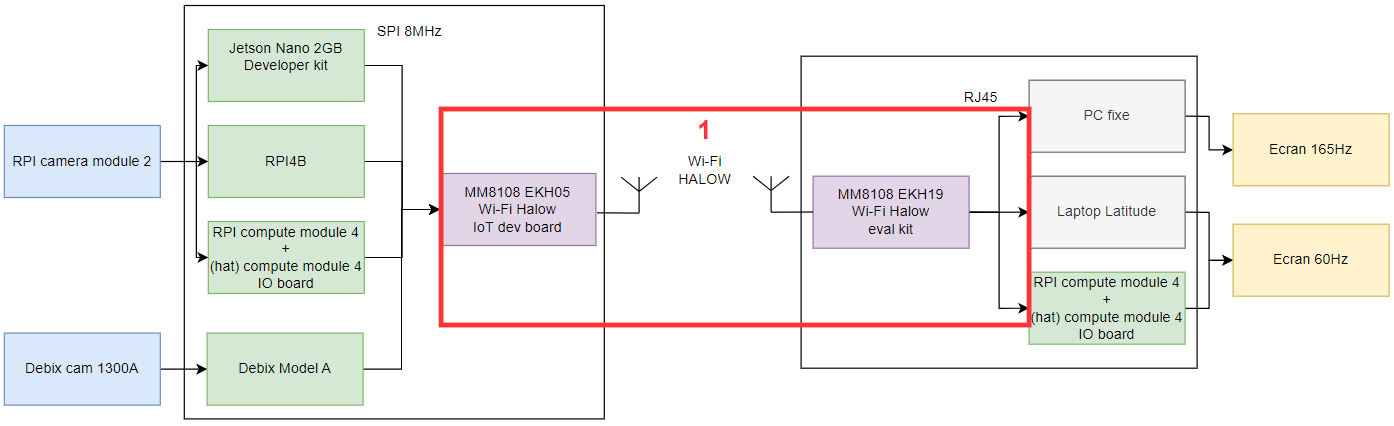
\includegraphics[width=1\textwidth]{imgs/complet_schematic_nb1.png}
    \caption{(1) Lien réseau Sub-1 GHz}
    \label{fig:complet_schematic_nb1}
\end{figure}

La norme IEEE 802.11 intègre intrinsèquement des mécanismes de fiabilité, tels que les accusés 
de réception (ACK) et les retransmissions automatiques, destinés à garantir l'intégrité des données. 
Cependant, dans le cadre d'un flux vidéo temps réel pour le FPV, la perte d'une trame est visuellement 
préférable à l'attente d'une retransmission, qui induit une latence beaucoup trop élevée. L'architecture 
réseau a donc été configurée pour s'affranchir de ces contraintes.

\subsection{Stratégie de transport UDP : Du Broadcast à l'Unicast optimisé}
Pour garantir la fluidité du flux vidéo, le protocole de transport UDP a été choisi en raison de son 
absence d'acquittements logiciels au niveau transport. Cependant, au niveau de la couche 
MAC\index{Couche MAC} (802.11), la gestion des acquittements matériels reste problématique.

\subsubsection{L'approche initiale : UDP Broadcast}
Dans un premier temps, l'application embarquée sur le STM32 ciblait une adresse IP de diffusion locale 
(\texttt{192.168.12.255}). En ciblant cette adresse, la couche réseau LwIP force l'en-tête Wi-Fi à 
utiliser l'adresse MAC \texttt{FF:FF:FF:FF:FF:FF}. Selon la norme 802.11, les trames diffusées à cette 
adresse ne déclenchent aucun acquittement (ACK) de la part des récepteurs. L'émetteur expédiait ainsi 
les paquets en flux tendu.

Cependant, une analyse métrologique approfondie a révélé un goulot d'étranglement caché inhérent aux 
points d'accès Wi-Fi : le DTIM (\textit{Delivery Traffic Indication Message}). Pour économiser l'énergie 
des clients, le routeur OpenWrt stocke temporairement les paquets \textit{Broadcast} en mémoire et 
attend le prochain signal de balise (Beacon) pour les envoyer groupés à vitesse réduite. Ce comportement 
standard induisait une latence allant jusqu'à 40 ms.

\subsubsection{La solution retenue : UDP Unicast et forçage de la QoS (WMM)}
Pour contourner la rétention du routeur, l'architecture réseau a basculé vers du \textbf{UDP Unicast}, ciblant directement l'adresse IP de la station de réception (ex: \texttt{192.168.12.10}). En Unicast, le point d'accès transmet la trame instantanément. 

Ce changement réintroduisant mécaniquement l'attente des acquittements MAC (ACKs), il a fallu paramétrer agressivement le modem radio pour que ces derniers ne détruisent pas la bande passante. Un "hack" de la Qualité de Service (QoS / WMM) a été implémenté au plus bas niveau :
\begin{enumerate}
    \item \textbf{Marquage IP (LwIP) :} Les paquets UDP vidéo sont marqués avec le type de service (TOS) le plus critique (\texttt{pcb->tos = 0xC0}, correspondant à la catégorie \textit{Voice}).
    \item \textbf{Écrasement des paramètres EDCA :} Dans le SDK Morse Micro, les paramètres d'accès au canal radio ont été forcés via la structure \texttt{mmwlan\_qos\_queue\_params}.
\end{enumerate}

\begin{lstlisting}[language=C]
// Configuration QoS ultra-agressive pour forcer le canal
struct mmwlan_qos_queue_params fpv_qos = {
    .aci = 3,         // ACI 3 = Voice (Priorite maximale)
    .aifs = 2,        // Temps d'attente inter-trame quasi-nul
    .cw_min = 1,      // Fenetre de contention minimale (parle tout de suite)
    .cw_max = 1,      // Relance immediate en cas de collision radio
    .txop_max_us = 0 
};
mmwlan_set_default_qos_queue_params(&fpv_qos, 1);
\end{lstlisting}

Grâce à cette configuration matérielle, le STM32 "écrase" virtuellement le reste du trafic réseau. Il s'accapare le canal instantanément pour expédier le flux vidéo, absorbant ainsi l'overhead des acquittements MAC sans accumuler de latence.

\subsection{Optimisation de la réactivité radio : Désactivation du PSM}
Par défaut, les modules Wi-Fi HaLow Morse Micro intègrent des mécanismes de gestion de l'énergie 
(\textit{Power Saving Mode}) destinés aux capteurs IoT sur batterie. Ce mode place la radio en 
veille entre les transmissions, ce qui induisait dans nos tests une latence systématique d'environ 
\textbf{22 ms} par paquet.

Pour un usage FPV, ce processus d'économie d'énergie n'est pas acceptable. Le mode veille a été explicitement désactivé 
dans le firmware du STM32 via l'appel suivant :
\begin{lstlisting}[language=C]
mmwlan_set_power_save_mode(MMWLAN_PS_DISABLED);
\end{lstlisting}
Cette modification a permis de stabiliser le temps de réponse réseau (\textit{ping}) entre \textbf{3 et 5 ms}, 
garantissant une gigue minimale.

\subsection{Contournement des contraintes réglementaires (ETSI vs FCC)}
Lors des premiers essais d'établissement de la liaison radio en MCS 1, une latence de base colossale 
d'environ 670 ms a été observée sur de simples paquets de test (Ping). 

L'analyse de ce délai a mis en évidence l'impact restrictif des normes réglementaires européennes (ETSI) 
régissant la bande des 868 MHz. Ces normes imposent un mécanisme de partage des ondes strict appelé 
\textit{Listen Before Talk} (LBT) ainsi que des restrictions de \textit{Duty Cycle} (temps d'émission 
maximal autorisé). Le module radio retenait intentionnellement les paquets pour respecter ces seuils 
légaux.

Afin d'évaluer les performances brutes du changement de MCS sans ces bridages logiciels imposés par la 
région, la configuration de l'émetteur et du récepteur a été basculée sur le domaine réglementaire 
américain (FCC, bande des 915 MHz). L'utilisation du Canal 27 (915.5 MHz) a permis de désactiver 
les mécanismes LBT, ramenant immédiatement la latence réseau de base à environ 27 ms pour des 
paquets de 1450 octets.

\subsection{Le routage et l'isolation IP (OpenWrt)}
Pour éviter les conflits de routage sur la station de réception, le réseau FPV est strictement isolé 
sur le sous-réseau \texttt{192.168.12.x}.

Lors de l'implémentation, un conflit IP majeur bloquait la transmission : le routeur OpenWrt (récepteur) 
possédait l'adresse \texttt{192.168.12.1} simultanément sur son interface Wi-Fi HaLow (\texttt{ahwlan}) 
et sur son interface Ethernet locale (\texttt{lan}). Pour résoudre ce conflit, il a suffi de migrer le 
LAN sur \texttt{192.168.13.1}.

Concernant le transfert des données à travers le routeur, une première approche a été 
testée : les paquets UDP entrants sur l'interface sans-fil étaient interceptés (via \texttt{tcpdump}) 
puis redirigés manuellement vers le port Ethernet à l'aide de l'utilitaire \texttt{netcat} (\texttt{nc}). 
Cependant, ce traitement en espace utilisateur (\textit{User-Space}) sollicitait lourdement le processeur 
du routeur et induisait une latence importante.
\begin{lstlisting}[language=bash]
tcpdump -i wlan0 -U -s 0 -w - "udp port 1337" | nc 192.168.12.10 9999
\end{lstlisting}

Pour optimiser le routage, un pont logiciel (\textit{Bridge}) a finalement été forcé au niveau du système 
d'exploitation du routeur :
\begin{lstlisting}[language=bash]
brctl addif br-ahwlan wlan0
\end{lstlisting}
Ce pont matériel permet au flux réseau en provenance de l'interface sans-fil de traverser le 
routeur et d'être répliqué directement sur le câble Ethernet (pour autant que la station de réception 
connectée soit sur le bon sous-réseau) sans être intercepté ni traité par la pile 
TCP/IP ou des utilitaires logiciels, économisant ainsi 10 à 20 ms de délai de traitement additionnel.

\subsection{Validation empirique et mathématique de la bande passante vidéo}
La désactivation de l'adaptation automatique de débit (\textit{Rate Control}) a été effectuée dans le 
SDK via la fonction ATE (\textit{Automated Test Equipment}, fonction utilisée en interne pour forcer 
des configurations matérielles spécifiques lors des phases de tests) :
\begin{lstlisting}[language=C]
mmwlan_ate_override_rate_control(MMWLAN_MCS_2, MMWLAN_BW_2MHZ, MMWLAN_GI_NONE);
\end{lstlisting}

En forçant l'utilisation du \textbf{MCS 2} sur une largeur de bande de \textbf{2 MHz}, la modulation 
employée (QPSK) garantit une excellente robustesse face aux obstacles physiques. Des mesures empiriques 
(par capture \texttt{tcpdump}) ont validé un débit utile réseau stable d'environ \textbf{1.34 Mbps} 
(soit une moyenne de 120 paquets de 1400 octets par seconde).

Il est ensuite nécessaire de confronter cette capacité physique aux exigences du flux vidéo. Le débit brut 
(non compressé) se calcule ainsi :
$$D_{brut} = W \times H \times F \times B_{pp}$$

Afin de contourner la rétention d'image du processeur de signal (ISP) de la caméra, la fréquence 
d'échantillonnage a dû être fixée à 60 FPS. Pour le flux vidéo retenu en résolution 480p 
(soit $640 \times 480$ pixels), capturé à 60 images par seconde et codé sur 24 bits de couleurs :
$$D_{brut\_480p60} = 640 \times 480 \times 60 \times 24 = 442\,368\,000 \text{ bps}$$
Soit environ 442.4 Mbps.

Un encodeur matériel moderne (H.264 / H.265), configuré pour du streaming en temps réel, offre un ratio de 
compression effectif standard avoisinant 1:200. Le débit réseau théorique requis deviendrait alors :
$$D_{cible} = \frac{D_{brut}}{C_{ratio}}$$
$$D_{cible\_480p60} = \frac{442.4 \text{ Mbps}}{200} \approx 2.21 \text{ Mbps}$$

Cette modélisation démontre clairement qu'à 60 images par seconde, même une résolution modeste de 480p avec 
une compression standard exigerait environ 2.21 Mbps, ce qui saturerait immédiatement le canal radio imposé 
par le MCS 2 (limité empiriquement à 1.34 Mbps).

C'est pour cette raison critique que l'encodeur matériel doit être paramétré de manière drastique. Afin de 
forcer ce flux à traverser la liaison radio tout en conservant une marge de sécurité vitale face aux baisses 
imprévisibles de la qualité du lien RF en condition de vol NLOS, le taux de compression final de l'encodeur 
a été bridé de manière stricte (CBR - \textit{Constant Bit Rate}) à \textbf{400 kbps}. 

\subsubsection{Impact de la compression sur la fragmentation des paquets}
Ce compromis de 400 kbps impose à l'encodeur un ratio de compression extrême (environ 1:1240) au détriment 
de la fidélité visuelle, mais garantit un avantage décisif sur la latence matérielle. En tenant compte du débit 
et de la fréquence d'échantillonnage (fréquence de capture d'image), le poids moyen d'une image vidéo compressée se calcule ainsi :
$$Taille_{image} = \frac{400\,000 \text{ bits/s}}{60 \text{ FPS} \times 8 \text{ bits}} \approx 833 \text{ octets}$$

Sachant que la charge utile maximale (MTU) définie pour nos trames UDP et nos transferts SPI est de 
\textbf{1400 octets}, l'écrasante majorité des images générées par l'encodeur tiennent dans 
\textbf{un seul et unique paquet réseau}. Cette caractéristique est fondamentale pour la basse latence : 
elle évite la fragmentation IP et exempte le récepteur de devoir stocker et attendre de multiples paquets 
pour reconstruire et décoder une seule trame vidéo.

Bien que cette caractéristique "zéro-fragmentation" ait constitué un atout majeur lors de nos premières 
itérations logicielles basées sur la compression H.264, le passage ultérieur au format MJPEG 
(détaillé dans la suite de ce document pour des raisons de latence d'encodage) réintroduira le défi 
de la fragmentation réseau UDP. Ce phénomène nécessitera une ingénierie logicielle spécifique au niveau 
du pont SPI pour reconstituer l'intégrité des trames sans pénaliser le temps réel.